\documentclass[border=10pt]{standalone}
\usepackage{pgfplots}
\pgfplotsset{compat=1.18}

\begin{document}
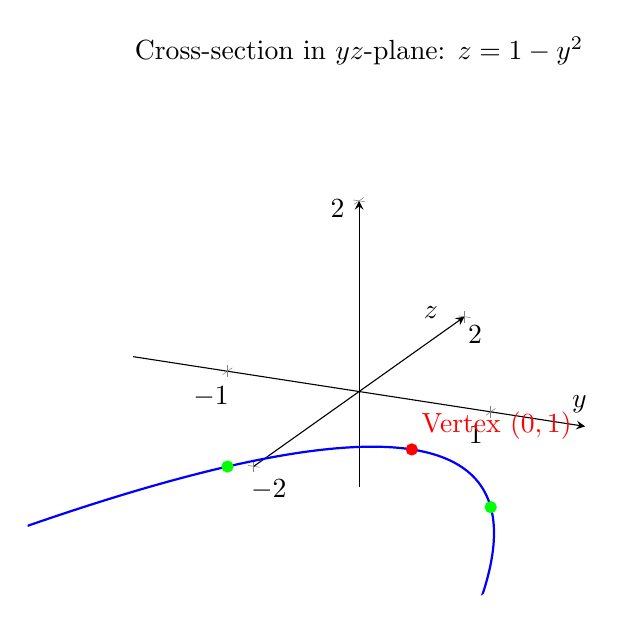
\begin{tikzpicture}
\begin{axis}[
    xlabel={$y$},
    ylabel={$z$},
    title={Cross-section in $yz$-plane: $z = 1 - y^2$},
    domain=-2:2,
    samples=100,
    grid=major,
    width=10cm,
    height=8cm,
    ymin=-2,
    ymax=2,
    zmin=-1,
    zmax=2,
    axis lines=center,
]
\addplot[blue, thick, domain=-2:2] {1 - x^2};
\addplot[red, only marks, mark=*] coordinates {(0,1)} node[above right] {Vertex $(0,1)$};
\addplot[green, only marks, mark=*] coordinates {(-1,0) (1,0)};
\end{axis}
\end{tikzpicture}
\end{document}